\section{信道容量的计算}

在4.3节我们给出了信道容量的定义并求出了一些特殊信道的容量,但对于一般的信道,求它的容量并不是件容易的事.在这一节中我们给出一些计算信道容量的方法.

\subsection{凸函数的极大值性质}

因为信道容量是互信息的最大值, 所以为了求得某个信道的容量, 先研究这个信道的输入和输出之间的互信息.如前所记, 信道的输入和输出字母表分别是
$$
\mathscr{U}=\left\{u_{1}, u_{2}, \cdots, u_{a}\right\} \quad \mathscr{V}=\left\{v_{1}, v_{2}, \cdots, v_{b}\right\},
$$
信道的转移概率矩阵 $ p\left(v_{j} \mid u_{i}\right) $ 给定. 因此信道容量的计算问题就是求
$$
I(\xi ; \eta)=I(p(u) ; p(v \mid u)) \quad p(u) \in \mathscr{P}_{\mathscr{U}}
$$
的最大值问题.

记入口分布 $ \overline{p}=\left\{p\left(u_{1}\right), p\left(u_{2}\right), \cdots, p\left(u_{a}\right)\right\} $,我们可以把互信息写成如下形式:
$$
I(\xi ; \eta)=\sum_{i=1}^{a} \sum_{j=1}^{b} p\left(u_{i}\right) p\left(v_{j} \mid u_{i}\right) \log \frac{p\left(v_{j} \mid u_{i}\right)}{\sum\limits_{\ell=1}^{a} p\left(u_{\ell}\right) p\left(v_{j} \mid u_{\ell}\right)} .
$$

\begin{lemma}
    对固定的转移概率 $ p(v \mid u) $, 互信息
$$
I(\overline{p})=I(p(u) ; p(v \mid u))
$$
是 $ \overline{p} $ 上的凸函数.
\end{lemma}
\begin{lemma}
    设 $ f(\overline{p}) $ 是有 $ n $ 个输入变量的连续上凸函数, 输入 $  \overline{p}=\left(p_{1}, p_{2}, \cdots, p_{a}\right) $ 满足
$$
\sum_{i=1}^{a} p_{i}=1, \quad p_{i} \geq 0, \quad i=1,2, \cdots, a
$$
且函数的偏导数 $ \partial f(\overline{p}) / \partial p_{i}, i=1,2, \cdots, a $ 有定义且连续, 则函数 $ f(\overline{p}) $ 对于 $ \overline{p}^{*}=\left(p_{1}^{*}, \cdots, p_{a}^{*}\right) $ 取最大值的充要条件为存在某一实数 $ \lambda $, 且满足
$$
\begin{array}{ll}
\dfrac{\partial f\left(\overline{p}^{*}\right)}{\partial p_{i}^{*}}=\lambda, & \text { 对 } p_{i}^{*}>0 \text { 的 } i, \\
\dfrac{\partial f\left(\overline{p}^{*}\right)}{\partial p_{i}^{*}} \leq \lambda, & \text { 对 } p_{i}^{*}=0 \text { 的 } i .
\end{array}
$$
\end{lemma}
\begin{remark}

(1)只需证明对于其他输入 $ \overline{p} $, 都有 $ f(\overline{p}) \leq f\left(\overline{p}^{*}\right) $
    
(2) 求函数极值的方法: 对 $ p_{i}^{*}>0 $ 的 $ i,\left.\dfrac{\partial f(\overline{p})}{\partial p_{i}}\right|_{\overline{p}=p^{*}}=\lambda $ 时, $ f(\overline{p}) $ 取得最大值.
\end{remark}


\subsection{信道容量的计算}
我们下面只讲用极值法求信道容量的方法, 利用迭代法求信道容量的方法不讲.

\begin{theorem}
    一个信道的入口分布 $ \overline{p}^{*}=\left(p^{*}\left(u_{1}\right), \cdots, p^{*}\left(u_{s}\right)\right) $ 使得输入和输出之间的互信息达到最大值的充要条件是存在一个常数 $ C $, 满足
$$
\begin{aligned}
\sum_{j=1}^{b} p\left(v_{j} \mid u_{i}\right) \log \frac{p\left(v_{j} \mid u_{i}\right)}{\sum\limits_{\ell=1}^{a} p^{*}\left(u_{\ell}\right) p\left(v_{j} \mid u_{\ell}\right)}&=C, \quad \text { 对于 } p^{*}\left(u_{i}\right)>0, \\
\sum_{j=1}^{b} p\left(v_{j} \mid u_{i}\right) \log \frac{p\left(v_{j} \mid u_{i}\right)}{\sum\limits_{\ell=1}^{a} p^{*}\left(u_{\ell}\right) p\left(v_{j} \mid u_{\ell}\right)} &\leq C, \quad \text { 对于 } p^{*}\left(u_{i}\right)=0 .
\end{aligned}
$$
这时 $ C $ 即为信道容量.
\end{theorem}
\begin{proof}
 令 $ I(\xi ; \eta)=I(p) $. 由引理 , 互信息达到信道容量的充要条件为存在一常数 $ \lambda $, 使得:
$$
\begin{aligned}
\left.\frac{\partial I(\overline{p})}{\partial p_{i}}\right|_{\overline{p}=p^{*}}=\lambda, \quad p_{i}^{*}>0, \\
\left.\frac{\partial I(\overline{p})}{\partial p_{i}}\right|_{\overline{p}=p^{*}} \leq \lambda, \quad p_{i}^{*}=0 . 
\end{aligned}
$$

$$I(\overline{p})=\sum_{i=1}^{a} \sum_{j=1}^{b} p\left(u_{i}\right) p\left(v_{j} \mid u_{i}\right) \log p\left(v_{j} \mid u_{i}\right)- 
\sum_{i=1}^{a} \sum_{j=1}^{b} p\left(u_{i}\right) p\left(v_{j} \mid u_{i}\right) \log \left(\sum_{\ell=1}^{a} p\left(u_{\ell}\right) p\left(v_{j} \mid u_{\ell}\right)\right)$$

对 $ p_{i}\left(p\left(u_{i}\right)\right) $ 求偏导,则其它的 $ p\left(u_{j}\right) $ 视为常数,求偏导为 0 .

$$ \begin{aligned} \frac{\partial I(\bar{p})}{\partial p_{i}}&= \sum_{j=1}^{b} p\left(v_{j} \mid u_{i}\right) \log p\left(v_{j} \mid u_{i}\right)-\sum_{j=1}^{b} p\left(v_{j} \mid u_{i}\right) \log \left(\sum_{\ell=1}^{a} p\left(u_{\ell}\right) p\left(v_{j} \mid u_{\ell}\right)\right) \\ &-\sum_{k=1}^{a} \sum_{j=1}^{b} p\left(u_{k}\right) p\left(v_{j} \mid u_{k}\right) \frac{p\left(v_{j} \mid u_{i}\right)}{\sum\limits_{\ell=1}^{a} p\left(u_{\ell}\right) p\left(v_{j} \mid u_{\ell}\right)} \\ &=\sum_{j=1}^{b} p\left(v_{j} \mid u_{i}\right) \log \frac{p\left(v_{j} \mid u_{i}\right)}{q\left(v_{j}\right)}-\sum_{j=1}^{b}\left(\sum_{k=1}^{a} p\left(u_{k}\right) p\left(v_{j} \mid u_{k}\right)\right) \frac{p\left(v_{j} \mid u_{i}\right)}{\sum\limits_{\ell=1}^{a} p\left(u_{\ell}\right) p\left(v_{j} \mid u_{\ell}\right)} \\ &=\sum_{j=1}^{b} p\left(v_{j} \mid u_{i}\right) \log \frac{p\left(v_{j} \mid u_{i}\right)}{q\left(v_{j}\right)}-\sum_{j=1}^{b} p\left(v_{j} \mid u_{i}\right) \frac{\sum\limits_{k=1}^{a} p\left(u_{k}\right) p\left(v_{j} \mid u_{k}\right)}{\sum\limits_{\ell=1}^{a} p\left(u_{\ell}\right) p\left(v_{j} \mid u_{\ell}\right)} \\ &=\sum_{j=1}^{b} p\left(v_{j} \mid u_{i}\right) \log \frac{p\left(v_{j} \mid u_{i}\right)}{q\left(v_{j}\right)}-\sum_{j=1}^{b} p\left(v_{j} \mid u_{i}\right) \\ &=\sum_{j=1}^{b} p\left(v_{j} \mid u_{i}\right) \log \frac{p\left(v_{j} \mid u_{i}\right)}{q\left(v_{j}\right)}-1\\
&=\sum_{j=1}^{b} p\left(v_{j} \mid u_{i}\right) \log \frac{p\left(v_{j} \mid u_{i}\right)}{\sum\limits_{\ell=1}^{a} p\left(u_{\ell}\right) p\left(v_{j} \mid u_{\ell}\right)}-1
\end{aligned} $$
令
$$
\lambda=\left.\frac{\partial I(\overline{p})}{\partial p_{i}}\right|_{p=p^{*}},
$$
则
$$
\lambda=\sum_{j=1}^{b} p\left(v_{j} \mid u_{i}\right) \log \frac{p\left(v_{j} \mid u_{i}\right)}{\sum\limits_{k=1}^{a} p_{k}^{*} p\left(v_{j} \mid u_{k}\right)}-1
$$
两边同时乘以 $ p_{i}^{*} $ 再对 $ i $ 求和有
$$
\begin{aligned}
\lambda & =\sum_{i=1}^{a} p_{i}^{*} \frac{\partial I(\overline{p})}{\partial p_{i}} \mid_{ p=p^{*}} \\
& =\sum_{i=1}^{a} \sum_{j=1}^{b} p_{i}^{*} p\left(v_{j} \mid u_{i}\right) \log \frac{p\left(v_{j} \mid u_{i}\right)}{\sum\limits_{k=1}^{a} p_{k}^{*} p\left(v_{j} \mid u_{k}\right)}-\sum_{i=1}^{a} p_{i}^{*} \\
& =\sum_{i=1}^{a} \sum_{j=1}^{b} p_{i}^{*} p\left(v_{j} \mid u_{i}\right) \log \frac{p\left(v_{j} \mid u_{i}\right)}{\sum\limits_{k=1}^{a} p_{k}^{*} p\left(v_{j} \mid u_{k}\right)}-1 \\
& =I\left(\bar{p}^{*}\right)-1=C-1
\end{aligned}
$$
根据第二个引理 $, I(\overline{p}) $ 在 $ \overline{p}^{*} $ 取最大值 $ I\left(\bar{p}^{*}\right), C=I\left(p^{*}\right)=\lambda+1 $.
$$
C=\sum_{j=1}^{b} p\left(v_{j} \mid u_{i}\right) \log \frac{p\left(v_{j} \mid u_{i}\right)}{\sum\limits_{\ell=1}^{a} p^{*}\left(u_{\ell}\right) p\left(v_{j} \mid u_{\ell}\right)}, \quad \text { 对于 } p^{*}\left(u_{i}\right)>0 \text {. }
$$
\end{proof}

\begin{example}
对于 $ M $ 信道, 它的信道矩阵为
$$
\left(\begin{array}{ccc}
1-p & 0 & p \\
0 & 1-p & p
\end{array}\right), \quad 0<p<1 .
$$
设入口分布为 $ \overline{p}=\left(p_{0}, p_{1}\right) $, 对应的出口分布为 $ \overline{q}=\left\{q_{0}, q_{1}, q_{2}\right\} $,而 $ q\left(v_{j}\right)=\sum\limits_{i=1}^{a} p\left(u_{i}\right) p\left(v_{j} \mid u_{i}\right) $.
由定理的结论知
$$
\begin{aligned}
C&=\sum_{j=1}^{b} p\left(v_{j} \mid u_{i}\right) \log \frac{p\left(v_{j} \mid u_{i}\right)}{\sum\limits_{\ell=1}^{a} p\left(u_{\ell}\right) p\left(v_{j} \mid u_{\ell}\right)}\\ & =\sum_{j=1}^{b} p\left(v_{j} \mid u_{i}\right) \log \frac{p\left(v_{j} \mid u_{i}\right)}{q\left(v_{j}\right)} \\
& =(1-p) \log \frac{1-p}{q_{0}}+p \log \frac{p}{q_{2}}  =(1-p) \log \frac{1-p}{q_{1}}+p \log \frac{p}{q_{2}}
\end{aligned}
$$
于是有 $ q_{0}=q_{1} $,
而
$$
\begin{aligned}
\left(q_{0}, q_{1}, q_{2}\right)  =\left(p_{0}, p_{1}\right)\left(\begin{array}{ccc}
1-p & 0 & p \\
0 & 1-p & p
\end{array}\right) =\left(p_{0}(1-p), p_{1}(1-p), p\right) .
\end{aligned}
$$
由 $ q_{0}=q_{1} $ 知, $ p_{0}=p_{1} \Rightarrow p_{0}=p_{1}=\frac{1}{2}, \quad q_{0}=q_{1}=\frac{1-p}{2}, q_{2}=p $,于是有 $ C=1-p $.
\end{example}


\section{信道的编码和译码问题}
在本章4.2节中,我们已给出了信道序列的可达速率的定义, 它的实质是存在适当的编码与译码算法, 使消息传递的误差很小, 而且可以转送一定数量的数据量.
我们现在给出一个关于信道序列的可达速率的等价条件. 我们仍记
$$
\mathscr{C}^{n}=\left(\mathscr{U}^{n}, p\left(v^{(n)}\right) \mid u^{(n)}, \mathscr{V}^{n}\right)
$$
为信道序列, 记 $ \mathscr{S}^{n}=\left\{\mathscr{X}^{n}, p^{(n)}\left(x^{n}\right)\right\} $ 为信源序列, 在4.1节中我们已经给出可达速率 $ R $ 的定义, 且取信源序列为 $ \mathscr{S}^{n} $
$$
\left\{\begin{array}{l}
\mathscr{X}^{n}=\mathscr{Y}^{n}=\left\{1,2, \cdots, M_{n}\right\}, \\
P^{(n)}\left(x^{(n)}\right)=\frac{1}{M_{n}}, \text { 对任何 } x^{(n)} \in \mathscr{X}^{n},
\end{array}\right.
$$
所给,那么信道的编码问题就是求信道序列的最大可达速率问题. 为讨论这个问题, 我们先给出 $ R $ 是可达速率的一个等价条件, 由这个等价条件也可看到信道的编码问题的本质.

\begin{definition}
    信道序列仍记为 $ \mathscr{C}^{n} $. 我们称
$$
\left(u_{i}^{(n)}, \mathscr{B}_{i}^{(n)}\right), i=1,2, \cdots, M_{n}
$$
是 $ \mathscr{C}^{n} $ 的一组 $ \epsilon $ 专线,如果它满足以下条件.

(1) $ u_{i}^{(n)} \in \mathscr{U}^{n} $, 它们互不相同.

(2) $ \mathscr{B}_{i}^{(n)} $ 是 $ \mathscr{V}^{n} $ 的一组子集, 它们互不相交, 即
$$
\mathscr{B}_{i}^{(n)} \cap \mathscr{B}_{j}^{(n)}=\emptyset \text {, 当 } i \neq j \text { 时, }
$$

(3)对任何 $ i=1,2, \cdots, M_{n} $, 有 $ P^{(n)}\left(\mathscr{B}_{i}^{(n)} \mid u_{i}^{(n)}\right)>1-\epsilon $ 成立.称式 中的 $ M_{n} $ 为 $ \epsilon $ 专线的数目.
\end{definition}

通过以下定理可以看到, $ \epsilon $ 专线与可达速率的关系问题.
\begin{theorem}
    $ R $ 是信道序列 $ \mathscr{C}^{n} $ 可达速率的充分与必要条件是存在数列 $ \epsilon_{n} \rightarrow 0 $, 使 $ \mathscr{C}^{n} $ 有 $ M_{n}>2^{n R\left(1-\epsilon_{n}\right)} $ 条 $ \epsilon_{n} $ 专线.
\end{theorem}
该定理不证明, 掌握结论.

具有 $ \epsilon_{n} $ 专线的编、译码的信息传输图如图所示.

\begin{figure}[h]
    \centering
    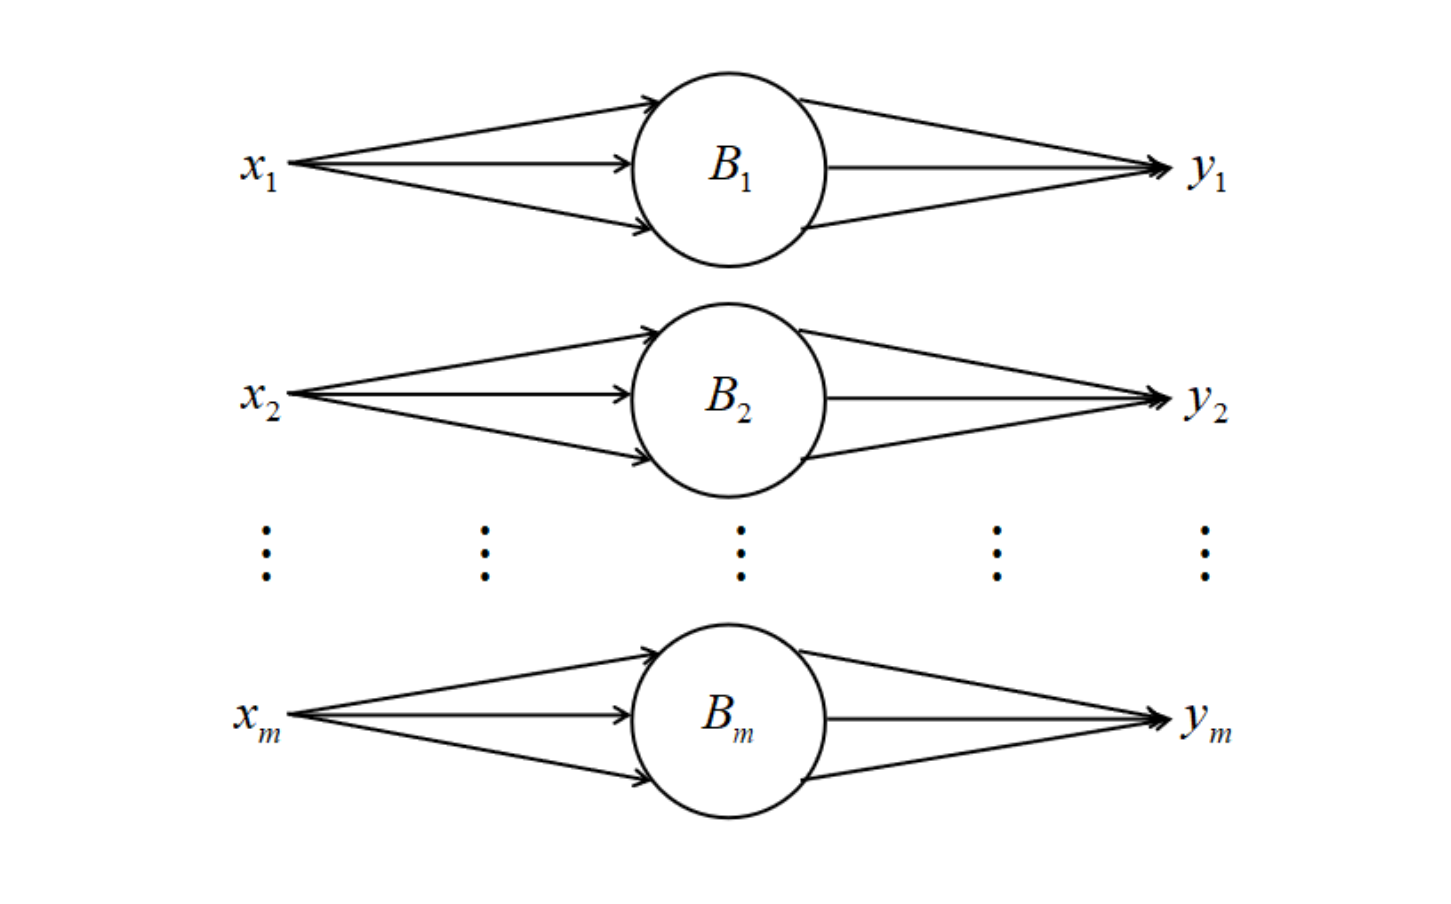
\includegraphics[width=0.5\linewidth]{image/7.png}
    \caption{$ \epsilon $ 专线的编码和译码判决方案表示图}
\end{figure}
可以看出, 专线对通信系统的编码和译码方式给出了一个形象的描述, 对我们理解通信编码问题很有帮助.


